\documentclass[conference]{IEEEtran}

% Class modification
\IEEEilabelindent=0pt

\usepackage[utf8]{inputenc}
\usepackage[x11names]{xcolor}

\usepackage[np]{numprint}

\definecolor{linkcolor}{RGB}{36,113,163}
\definecolor{citecolor}{RGB}{17,122,101}
\definecolor{urlcolor}{RGB}{148,39,38}

\usepackage[
    colorlinks,
    linkcolor=linkcolor,
    citecolor=citecolor,
    urlcolor=urlcolor
]{hyperref}

\usepackage{algorithm}
\usepackage{algpseudocode}

\usepackage{amsmath, amsfonts}

\usepackage{lipsum}

\usepackage{tikz}
\usetikzlibrary{decorations.pathreplacing, patterns}
\usetikzlibrary{calc, backgrounds}

\usepackage{xspace}

\usepackage{listings}

\lstset{
    basicstyle=\ttfamily,
    keywordstyle={[1]\color{Blue4}\bfseries}, % keywords style
    % keywordstyle={[2]\color{Pink4}}, % type style
    % keywordstyle={[3]\color{OrangeRed3}}, % function style
    % literate =
    %     {=>}{{=>}}2
    %     {/=}{{/=}}2,
    commentstyle=\itshape\color{gray}
}

\def\spark#1{\lstinline[language=Ada]{#1}}


\def\todo#1{\textcolor{red}{[#1]}}

\def\state#1{\textsf{\MakeUppercase{#1}}\xspace}
\def\sclosed{\state{closed}}
\def\ssynsent{\state{syn-sent}}
\def\ssynrcv{\state{syn-rcvd}}
\def\slisten{\state{listen}}
\def\sestab{\state{established}}
\def\sfwone{\state{fin-wait-1}}
\def\sfwtwo{\state{fin-wait-2}}
\def\sclosing{\state{closing}}
\def\sclosew{\state{close-wait}}
\def\slastack{\state{last-ack}}
\def\stimewait{\state{time-wait}}

\def\flag#1{\textsf{#1}\xspace}
\def\syn{\flag{SYN}}
\def\ack{\flag{ACK}}
\def\rst{\flag{RST}}
\def\fin{\flag{FIN}}

\let\code\texttt

\begin{document}

\title{Verification of a TCP/IP stack}

\author{%
\IEEEauthorblockN{Guillaume Cluzel}
\IEEEauthorblockA{\textit{Adacore \& ENS de Lyon}}
\and
\IEEEauthorblockN{Kyriakos Georgious}
\IEEEauthorblockA{\textit{Adacore \& University of Bristol}}
\and
\IEEEauthorblockN{Yannick Moy}
\IEEEauthorblockA{\textit{Adacore}}
\and
\IEEEauthorblockN{Clément Zeller}
\IEEEauthorblockA{\textit{Oryx Embedded}}
}

\maketitle

\begin{abstract}
\todo{Write the abstract.}
\end{abstract}

\begin{IEEEkeywords}
Network protocols,
deductive verification.
\end{IEEEkeywords}

\section{Introduction}

The usage of IoT devices has been put more within everyone's reach. Their
vulnerability is a major cause for concern, and as their number
increases, the number of attacks they suffer increases, putting at risk
the security of the owner's data collected by the object. \todo{Try to find a
relevant ref. I have found examples about the possibility to leak personnal data
on Google home/Alexa}.

The core of the IoT devices is built on top of the TCP protocol~\cite{rfc793} as
it is the most widely protocol used on the Internet, as the underlying protocol
for application layers such as HTTP, FTP or TLS. TCP is based on the underlying
IP protocol which is itself based on a link layer such as Ethernet. This
stacking of protocols is referred to as the TCP/IP stack.

Given the importance of the TCP protocol in network communications, some
researchers have attempted to formalize the protocol to either prove key
properties~\cite{smith1996formal} or even to fully prove the correctness of an
implementation against a complete specification~\cite{ridge2008rigorous}.
This latter implementation was performed in the HOL proof assistant, and while
the authors note that it would be possible in theory to extract an
implementation in Haskell from this work, this has not been adopted in practice.
The formalization of TCP specification and verification of a TCP implementation
face two difficulties:
RFC 793 is written in English, leaving many parts underspecified; the TCP
protocol is inherently concurrent which makes it complex to specify and verify.
As a result, there is currently no formally verified implementation for TCP that
is usable in industry.

Other communication protocols have been formalized in recent years, leading to a
formally verified implementation. The most prominent project in this area is the
Everest project~\cite{bhargavan2017everest}, which led to a formally verified
implementation in F* of TLS called miTLS~\cite{bhargavan2013implementing}. The
approach of the Everest project is to implement TLS in F*, a programming
language targeted at formal program verification.
Note that miTLS still relies on an untrusted implementation of TCP, and thus
could benefit from the results of our work.
This approach is often difficult to adopt in industry, as codebases are evolved
incrementally rather than replaced, both for economical and practical reasons.

Our approach in this work has been to incrementally evolve an existing TCP/IP
stack in C by replacing parts of the code with formally verified code in SPARK.
The stack chosen, CycloneTCP\footnote{\url{https://www.oryx-embedded.com/products/CycloneTCP.html}},
a mature TCP/IP stack targeted at embedded processors with no Operating System.
We present the TCP protocol in section~\ref{sec:TCP} and then briefly the
choosen stack, the Oryx Embedded one, in section~\ref{sec:stack}
before presenting the specification techniques used in section~\ref{sec:spec}
and then in sections~\ref{sec:verif} and~\ref{sec:API} we explain how we
formally implemented in SPARK the TCP user functions and how we hardened the
user's API. Finally we end in section~\ref{sec:results} by showing the results
of our work.



\section{TCP protocol}
\label{sec:TCP}

Initially described by the ``fathers of the Internet'' Vincent Cerf and Bob
Kahn, the TCP protocol was standardized in 1981 by RFC 793~\cite{rfc793}.
Its sturdiness makes it still one of the most widely used protocols today with
UDP.

In the OSI networking communication model, the TCP protocol is central and
located in the \emph{Transport layer}. It itself uses the \emph{Network layer}
to work.
The security of the \emph{Application} protocols depends on the security of
the \emph{Session layer} and consequently on the security of the TCP and UDP
protocols. Figure~\ref{Fig:TcpStack} gives an overview of how protocols are
stacked.

The purpose of this section is to give enough context to enable the reader to
follow the work conducted in this article.
The TCP protocol is connection-oriented in the sense that a connection requires
to be established between the two processes that exchange data.
The protocol is governed by a state machine described in
figure~\ref{Fig:statemachine}.
The implementation is rather free and lots of choices are left to the
programmer. However, the implementation must ensure some properties to be able
to communicate with other TCPs.


\begin{figure}[t]
    {\centering\scalebox{.55}{
    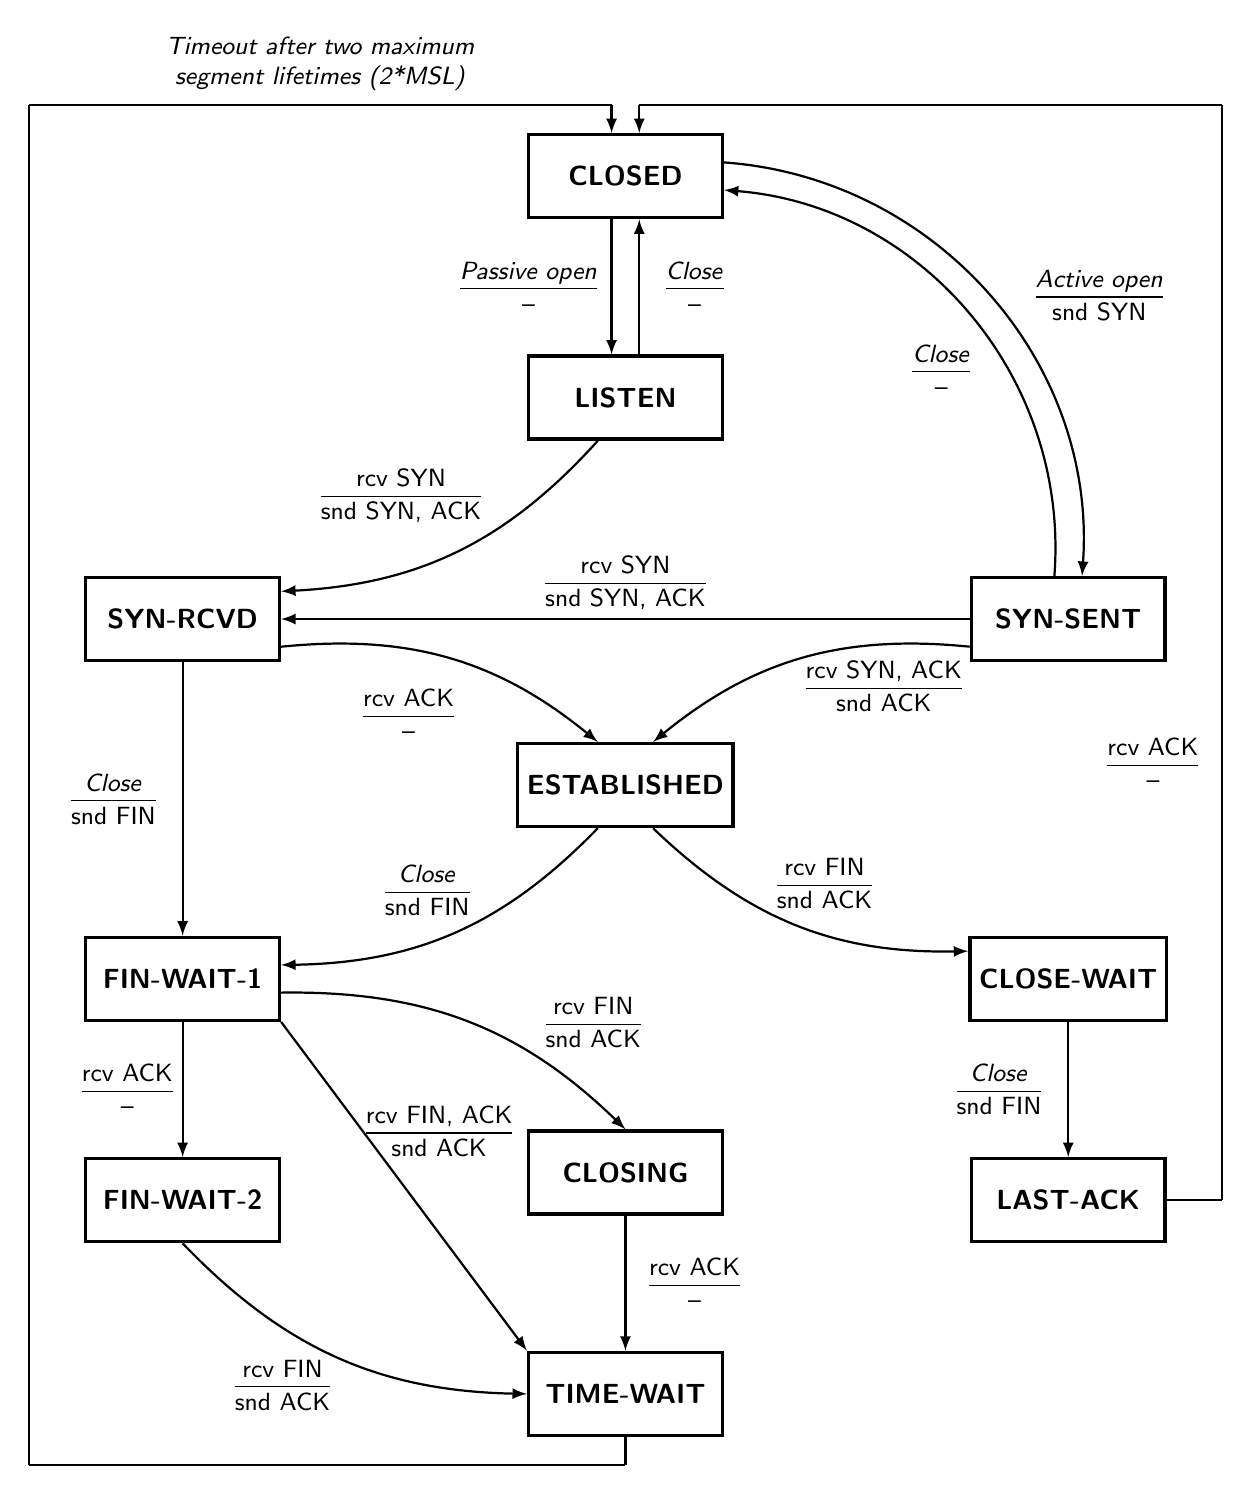
\begin{tikzpicture}[>=latex]
        \def\tfrac#1#2{\ensuremath{\displaystyle\frac{\text{\small#1}}{\text{\small#2}}}}
        %
        % Styles for states, and state edges
        %
        \tikzstyle{state} = [draw, very thick, fill=white, rectangle, minimum height=3em, minimum width=7em, node distance=8em, font={\sffamily\bfseries}]
        \tikzstyle{stateEdgePortion} = [black,thick];
        \tikzstyle{stateEdge} = [stateEdgePortion,->];
        \tikzstyle{edgeLabel} = [pos=0.5, text centered, font={\sffamily\small}];

        %
        % Position States
        %
        \node[state, name=closedStart] {CLOSED};
        \node[state, name=listen, below of=closedStart] {LISTEN};
        \node[state, name=synSent, below of=listen, right of=listen, xshift=8em] {SYN-SENT};
        \node[state, name=synRcvd, below of=listen, left of=listen, xshift=-8em] {SYN-RCVD};
        \node[state, name=established, below of=listen, node distance=14em] {ESTABLISHED};
        \node[state, name=finWait1, below of=established, left of=established, node distance=7em, xshift=-9em] {FIN-WAIT-1};
        \node[state, name=finWait2, below of=finWait1] {FIN-WAIT-2};
        \node[state, name=closeWait, below of=established, right of=established, node distance=7em, xshift=9em] {CLOSE-WAIT};
        \node[state, name=closing, below of=established, node distance=14em] {CLOSING};
        \node[state, name=lastAck, below of=closeWait] {LAST-ACK};
        \node[state, name=timeWait, below of=closing] {TIME-WAIT};

        %
        % Connect States via edges
        %
        \draw ($(closedStart.south) + (-.5em,0)$)
        edge[stateEdge] node[edgeLabel, xshift=-3em]{\tfrac{\emph{Passive open}}{--}}
        ($(listen.north) + (-.5em,0)$);
        \draw ($(listen.north) + (.5em,0)$)
        edge[stateEdge] node[edgeLabel, xshift=2em]{\tfrac{\emph{Close}}{--}}
        ($(closedStart.south) + (.5em,0)$);

        \draw ($(listen.south) + (-1em,0)$)
        edge[stateEdge, bend left=22.5] node[edgeLabel, xshift=-2em, yshift=2em]{\tfrac{rcv SYN}{snd SYN, ACK}}
        ($(synRcvd.east) + (0,1em)$);

        % \draw ($(synRcvd.north) + (.5em,0)$)
        % edge[stateEdge, bend left=45] node[edgeLabel,xshift=-4em]{\emph{Timeout}/RST}
        % ($(closedStart.west) + (0,-.5em)$);

        \draw ($(synSent.north) + (-.5em,0)$)
        edge[stateEdge, bend right=45] node[edgeLabel,xshift=-1em, yshift=-2em]{\tfrac{\emph{Close}}{--}}
        ($(closedStart.east) + (0,-.5em)$);
        \draw ($(closedStart.east) + (0,.5em)$)
        edge[stateEdge, bend left=45] node[edgeLabel,xshift=4em]{\tfrac{\emph{Active open}}{snd SYN}}
        ($(synSent.north) + (.5em,0)$);

        \draw (synSent.west)
        edge[stateEdge] node[edgeLabel, yshift=1.3em]{\tfrac{rcv SYN}{snd SYN, ACK}}
        (synRcvd.east);
        \draw (synRcvd)
        edge[stateEdge] node[edgeLabel, xshift=-2.5em]{\tfrac{\emph{Close}}{snd FIN}}
        (finWait1);

        \draw ($(synRcvd.east) + (0,-1em)$)
        edge[stateEdge, bend left=22.5] node[edgeLabel, xshift=-1.5em, yshift=-2em]{\tfrac{rcv ACK}{--}}
        ($(established.north) + (-1em,0)$);
        \draw ($(synSent.west) + (0,-1em)$)
        edge[stateEdge, bend right=22.5] node[edgeLabel, xshift=3em, yshift=-1em]{\tfrac{rcv SYN, ACK}{snd ACK}}
        ($(established.north) + (1em,0)$);

        \draw ($(established.south) + (-1em,0)$)
        edge[stateEdge, bend left=22.5] node[edgeLabel, xshift=-1em, yshift=1.5em]{\tfrac{\emph{Close}}{snd FIN}}
        ($(finWait1.east) + (0,.5em)$);
        \draw ($(established.south) + (1em,0)$)
        edge[stateEdge, bend right=22.5] node[edgeLabel, xshift=1em, yshift=1.5em]{\tfrac{rcv FIN}{snd ACK}}
        ($(closeWait.west) + (0,1em)$);

        \draw (finWait1.south)
        edge[stateEdge] node[edgeLabel, xshift=-2em]{\tfrac{rcv ACK}{--}}
        (finWait2.north);
        \draw ($(finWait1.east) + (0,-.5em)$)
        edge[stateEdge, bend left=22.5] node[edgeLabel, yshift=0em, xshift=4.5em]{\tfrac{rcv FIN}{snd ACK}}
        (closing.north);
        \draw (finWait1.south east)
        edge[stateEdge] node[edgeLabel, xshift=0em, yshift=2em, text width=3em]{\tfrac{rcv FIN, ACK}{snd ACK}}
        (timeWait.north west);

        \draw (finWait2.south)
        edge[stateEdge, bend right=22.5] node[edgeLabel, xshift=-2em, yshift=-1em]{\tfrac{rcv FIN}{snd ACK}}
        (timeWait.west);

        \draw (closing)
        edge[stateEdge] node[edgeLabel, xshift=2.5em]{\tfrac{rcv ACK}{--}}
        (timeWait);

        \draw (closeWait)
        edge[stateEdge] node[edgeLabel,xshift=-2.5em]{\tfrac{\emph{Close}}{snd FIN}}
        (lastAck);

        %
        % Connect lastAck to closed is slightly more complicated
        % no direct line-of-sight, so we need to take the scenic route
        %
        \coordinate (lastAck2ClosedA) at ($(lastAck.east) + (2em,0)$);
        \coordinate (lastAck2ClosedB) at ($(closedStart.north -| lastAck.east) + (2em,1em)$);
        \coordinate (lastAck2ClosedC) at ($(closedStart.north) + (0.5em,1em)$);
        \draw (lastAck.east) edge[stateEdgePortion] (lastAck2ClosedA);
        \draw (lastAck2ClosedA) edge[stateEdgePortion] node[edgeLabel,xshift=-2.5em, yshift=-4em]{\tfrac{rcv ACK}{--}} (lastAck2ClosedB);
        \draw (lastAck2ClosedB) edge[stateEdgePortion] (lastAck2ClosedC);
        \draw (lastAck2ClosedC) edge[stateEdge] ($(closedStart.north) + (0.5em,0)$);

        %
        % likewise for timeWait to closed
        %
        \coordinate (timeWait2ClosedA) at ($(timeWait.south) + (0,-1em)$);
        \coordinate (timeWait2ClosedB) at ($(timeWait.south -| finWait2.west) + (-2em,-1em)$);
        \coordinate (timeWait2ClosedC) at ($(closedStart.north -| finWait2.west) + (-2em,1em)$);
        \coordinate (timeWait2ClosedD) at ($(closedStart.north) + (-0.5em,1em)$);
        \draw (timeWait.south) edge[stateEdgePortion] (timeWait2ClosedA);
        \draw (timeWait2ClosedA) edge[stateEdgePortion] (timeWait2ClosedB);
        \draw (timeWait2ClosedB) edge[stateEdgePortion] (timeWait2ClosedC);
        \draw (timeWait2ClosedC) edge[stateEdgePortion]
        node[edgeLabel, text width=12.25em, yshift=1.5em]{\emph{Timeout after two maximum segment lifetimes (2*MSL)}}
        (timeWait2ClosedD);
        \draw (timeWait2ClosedD) edge[stateEdge] ($(closedStart.north) + (-0.5em,0)$);

        % draw dotted lines around passive and active closes
        % \begin{pgfonlayer}{background}
        %     \draw [join=round,black,dotted] ($(closeWait.north west) + (-1em, -1em)$) rectangle ($(lastAck.south east) + (1em, 1em)$);
        %     \draw [join=round,black,dotted] ($(finWait1.north west) + (-1em, -1em)$) rectangle ($(timeWait.south east) + (1em, 1em)$);
        % \end{pgfonlayer}

    \end{tikzpicture}}\par}
    \caption{TCP state machine.}
    \label{Fig:statemachine}
\end{figure}


\subsection{States}

Generally, every TCP communication session will go through the following three
phases (if no error occurs): 1)~opening the connection 2)~sending and receiving
the data and 3)~closing the connection.

The behavior of the three-phase communication can be described by the state
machine.
Every group of states corresponds to a one phase. More precisely \sclosed
stands for a closed connection. Both states \ssynsent and \ssynrcv denotes the
state that a TCP process can take during the initiation of a new connection. The
state \sestab represents the state when the connection is established,
\textit{i.e.} when two TCPs can communicate by sending and receiving data.
Then, two groups of states can be distinguished: the group formed by \sfwone,
\sfwtwo, \sclosing and \stimewait and that represents the state that a TCP can
reach when it is closing its connection and it is at the origin of the closing;
and the group formed by the state \sclosew and \slastack when the connection is
closing and the closing was initiated by the remote TCP.
Finally, the state \slisten stands for a TCP that is waiting for an incoming
connection.

\subsection{Flags}

The transition between the states are dictated by three things: user
actions, the reception of flags and timers. When a transition is triggered, a
response is given by sending of flags. The user actions, written in italic in
the automaton, can be an active or passive opening, or a close.
The corresponding user functions are detailed in the next paragraph.
The main flags that can be sent appear in figure~\ref{Fig:statemachine}.
They are sent alongside TCP segments, in the header.

The \syn flag is sent to synchronize two TCPs when they want to initiate a
connection. With a \ack flag, the last message received by the sender is
acknowledged. \fin is sent when a TCP wants to close the connection.
Moreover, a flag named \rst can be sent or received at any time and it forces the
connection to be reset. If so, both TCPs jump to the state \sclosed.

The state machine in figure~\ref{Fig:statemachine} does not reflect
error-conditions or any action which are not connected with the state changes.
Rather, it gives an overview of all the possible states a TCP connection could
reach over its lifetime. The transition are represented in the format
$\frac{\ \ x \ \ }{\ \ y \ \ }$ where $x$ is the event that triggers the
transition and $y$ is the response given to fulfil the transition.


\subsection{User functions}

In order to use the TCP protocol in programs, the nom defines user functions that
can be invoked by the software programmer in his code. This is the well-known
\emph{socket API}, available on almost all operating systems and known on POSIX
systems as the Berkeley sockets. This API specifies the already mentioned
\code{open} and \code{close} functions, as well as functions \code{send} and
\code{receive} to send or receive data once the connection is opened. The
behavior of each function is defined depending on the state of the TCP when the
function is called.
Even if user functions can initiate a change of state, it appears in the state
machine that most of transition are initiated by the reception of flags.

\subsection{Tasks}

A model with multiple tasks is adopted in the norm. Each task has a dedicated
job. One task is dedicated to the sending and the reception of messages. Another
is dedicated to the user functions and the last to the timers. Timers can resend
data or close a connection if the remote server does not acknowledged a message.
The first task mentioned performs most of the transitions.

\section{CycloneTCP library}
\label{sec:stack}

\newlength\hatchdistance
\hatchdistance=10pt
\pgfdeclarepatternformonly[\hatchdistance,2pt]{north east hatch}% name
    {\pgfqpoint{-1pt}{-1pt}}% below left
    {\pgfqpoint{\hatchdistance}{\hatchdistance}}% above right
    {\pgfpoint{\hatchdistance-1pt}{\hatchdistance-1pt}}%
    {
        \pgfsetcolor{orange!40}
        \pgfsetlinewidth{2pt}
        \pgfpathmoveto{\pgfqpoint{0pt}{0pt}}
        \pgfpathlineto{\pgfqpoint{\hatchdistance}{\hatchdistance}}
        \pgfusepath{stroke}
    }
\begin{figure}[t]
    \centering\begin{tikzpicture}[x=.12\linewidth,y=.45cm,
        application/.style={font=\sffamily\tiny,
                            draw,
                            minimum width=.115\linewidth,
                            minimum height=.4cm},
        session/.style={font=\sffamily\tiny,
                        draw,
                        minimum width=.715\linewidth,
                        minimum height=.4cm},
        transport/.style={font=\sffamily\tiny,
                          draw,
                          minimum width=.295\linewidth,
                          minimum height=.4cm},
        network/.style={font=\sffamily\tiny,
                        draw,
                        minimum width=.355\linewidth,
                        minimum height=.4cm},
        datalink/.style={font=\sffamily\tiny,
                         draw,
                         minimum width=.139\linewidth,
                         minimum height=.4cm}
    ]
        \node[application] at (0,10) {HTTP};
        \node[application] at (1,10) {HTTP/2};
        \node[application] at (2,10) {MQTT};
        \node[application] at (3,10) {MQTT-SN};
        \node[application] at (4,10) {CoAP};
        \node[application] (CoinA) at (5,10) {FTP};
        \node[application] at (0,9)  {SMTP};
        \node[application] at (1,9)  {SNTP};
        \node[application] at (2,9)  {DNS};
        \node[application] at (3,9)  {NetBIOS};
        \node[application] at (4,9)  {SNMPv3};
        \node[application] at (5,9)  {TFTP};
        \node[application, minimum width=.235\linewidth] at (.5,8) {WebSocket};
        \node[application] at (2,8)  {mDNS};
        \node[application] at (3,8)  {DNS-SD};
        \node[application] at (4,8)  {DHCP};
        \node[application] (CoinB) at (5,8)  {DHCPv6};
        \node[session, fill=green!70!yellow!20] (Socket) at (2.5, 7) {Socket};
        \node[transport, preaction={fill, green!70!yellow!20}, pattern=north east hatch, pattern color=orange!40] at (.75,6) {TCP};
        \node[transport, fill=orange!40] at (3.25,6) {UDP};
        \node[application, fill=orange!40] (RAW) at (5,6) {RAW};
        \node[network, fill=orange!40] at (1, 5) {IPv4};
        \node[network, fill=orange!40] (IPv6) at (4, 5) {IPv6};
        \node[application, fill=orange!40] at (0,4) {ARP};
        \node[application, fill=orange!40] at (1,4) {Auto-IP};
        \node[application, fill=orange!40] at (2,4) {NDP};
        \node[application, fill=orange!40] at (3,4) {SLAAC};
        \node[application, fill=orange!40] (ICMP) at (4,4) {ICMP};
        \node[application, fill=orange!40] (MLDv1) at (5,4) {MLDv1};
        \node[datalink, fill=orange!40] at (0.10, 3) {Ethernet};
        \node[datalink, fill=orange!40] at (1.3, 3) {Wi-Fi};
        \node[datalink, fill=orange!40] at (2.5, 3) {PPP};
        \node[datalink, fill=orange!40] at (3.7, 3) {USB/RNDIS};
        \node[datalink, fill=orange!40] (G3) at (4.9, 3) {G3-PLC};


        \draw[decorate, decoration={brace}, line width=.5pt]
            ([xshift=2pt]CoinA.north east) -- ([xshift=2pt]CoinB.south east)
            node [midway, anchor=west, font=\sffamily\tiny] {Application layer};
        \draw[decorate, decoration={brace}, line width=.5pt]
            ([xshift=2pt]Socket.north east) -- ([xshift=2pt]Socket.south east)
            node [midway, anchor=west, font=\sffamily\tiny] {Session layer};
        \draw[decorate, decoration={brace}, line width=.5pt]
            ([xshift=2pt]RAW.north east) -- ([xshift=2pt]RAW.south east)
            node [midway, anchor=west, font=\sffamily\tiny] {Transport layer};
        \draw[decorate, decoration={brace}, line width=.5pt]
            ([xshift=2pt]IPv6.north east) -- ([xshift=2pt]MLDv1.south east)
            node [midway, anchor=west, font=\sffamily\tiny] {Network layer};
        \draw[decorate, decoration={brace}, line width=.5pt]
            ([xshift=2pt]G3.north east) -- ([xshift=2pt]G3.south east)
            node [midway, anchor=west, font=\sffamily\tiny] {Data Link layer};
    \end{tikzpicture}

    \caption{Overview of the TCP/IP CycloneTCP stack in the OSI model. Green parts represent
             what have been translated in SPARK and in orange the underlying untrusted part written in C.}
    \label{Fig:TcpStack}
\end{figure}

CycloneTCP is a professional-grade embedded TCP/IP library developed by the
Oryx Embedded company. It provides several network protocols whose implementations
are meant to conform with the Request for Comments (RFC) Internet standards.
Figure~\ref{Fig:TcpStack} shows the protocols implemented in the library.
These include the IPv4 or Ipv6 of the network layer, TCP and UDP of the transport
layer and, among other, DHCP and HTTP of the application layer.
In particular, the TCP implementation is conform with the RFC 793
norm~\cite{rfc793}.

The library is written in ANSI C, and it supports a large number of 32-bits
embedded processors and a large number of Real-time Operating System (RTOS).
Hence, a model based on multiple tasks has been adopted to implement the TCP
protocol as described in the norm, with, in addition, complex cooperation
mechanisms. A task is dedicated to the user code, another to the timers and the
last is assigned to the processing of the incoming segments.
It can also run on bare metal environment.

The quality of the C implementation hailed in the AMNESIA:33 report~\cite{AMNESIA33}
as one of the most resilient TCP/IP stack. This gives a really good assurance
in the code and it strengthens the confidence that we can have in a formally
verified code running inside the library environment.
\todo{Add anything else relevant about the CycloneTCP library}.



\section{Specification techniques used}
\label{sec:spec}

\subsection{The SPARK programming language}

Ada is a general-purpose procedural programming language. The design of the Ada
language puts great emphasis on the safety and correctness of the program. This
objective is realized by using a readable syntax that uses keywords instead of
symbols where reasonable. The type system is strong and strict and many
potential violations of type constraints can be detected statically by the
compiler. If not, a run-time check is inserted into the program, to guarantee
the detection of incorrect situations. Ada 2012 introduced contract based
programming to Ada. In particular, it is possible to attach pre- and
postconditions to subprograms\footnote{In Ada, a distinction is made between
  functions that return a value, and procedures, which do
  not. \emph{Subprogram} is the term that designates both.}.  These conditions
can be checked during the execution of the program, just like assertions.

SPARK~\cite{mccormick2015building} is the name of a platform that provides
formal verification for Ada. It uses the user-provided contracts and attempts
to prove that the runtime checks cannot fail and that postconditions are
established by the corresponding subprograms.  As formal verification for the
whole Ada language would be intractable, SPARK is also the name of the subset
of the Ada language that is supported by the SPARK tool called
GNATprove\footnote{\url{http://docs.adacore.com/spark2014-docs/html/ug/}}.
This subset contains almost all features of Ada, though sometimes in a
restricted form.  In particular, expressions should be free from side effects,
and aliasing is forbidden (no two variables should share the same memory
location or overlap in memory), including when using pointers thanks to the use
of an ownership policy~\cite{dross2020recursive}.  This restriction greatly
simplifies the memory model used in the SPARK tool: any program variables can
be reasoned about independently from other variables.

GNATprove performs two kinds of analysis modularly on individual subprograms:
information flow to detect reads of uninitialized data and violations of flow
contracts; deductive verification based on the Why3 platform to generate
verification conditions for SMT solvers via a weakest-precondition calculus to
detect possible runtime errors and violations of functional contracts.

\subsection{Interfacing SPARK and C code}

To reduce the size of the work, only few functions of interest have been
translated in SPARK. Most of the C code has been kept.
Hopefully, SPARK integrates a mechanism to interface C code. No verification are
performed on the C code, but pre- and postconditions can be attached to
subprograms and they can be called in SPARK code.
The functional specification are not proved, thus it is the role of the
programmer to ensure the correctness of the contracts.

The types in SPARK can be more expressive than the types in C which adds more
safety to the SPARK code.
But the C and the SPARK code can share objects and it is essential that the
memory representations of an object are the same in the C and in the SPARK side.
For instance, if a C function is supposed to be called with a 32-bits integer,
it is the responsibility of the programmer to ensure that the function is
actually called with a 32-bits integer in the SPARK code.

Interfacing C and SPARK code is a great opportunity to plug our work in an
existing library, but it is also be a source of errors if it is not done
carefully. In section~\ref{sec:verif} it is explain how we have dealt with these
problems to ensure the quality of our work.

\subsection{Dealing with pointers}
\label{sec:pointers}

In CycloneTCP library, pointers are often manipulated at top-level and transmitted
to C functions. They are also used as fields in structures, for instance in
the socket structure to store other complex data-structures and recursive pointer
based data-structures. SPARK use a pointer ownership model to prevent bugs
involving pointers such as memory leak or double free. When a memory area is
allocated, a pointer points to this memory area and thus it is owned.
The ownership of the memory can be moved but the memory must be deallocated
before the end of the execution of the program.

\subsection{Specifying the frame condition}

The socket structure is shared between different functions, and contains a lot
of fields. Most of the fields are used in other parts of library and are not
relevant for our verification. We only need to concentrate on a subset of fields
to make the specifications easier to write, and to understand.
This can be achieve in SPARK by using \emph{models} and \emph{ghost code}.
The ghost code is code uses by GNATprove to simplify the proof that is removed
by the compiler to keep the size of executable file reasonable.

In the contract, we use the construction \spark{Model(Sock)} to refer the
relevant fields of the object \spark{Sock} where
\spark{Model} is a ghost function that extract the fields of interest from
\spark{Sock}, like in the construction frequently used in postconditions
\begin{lstlisting}[language=Ada, basicstyle=\small\ttfamily]
Model(Sock) = (Model(Sock)'Old with delta
                    State => TCP_STATE_CLOSED)
\end{lstlisting}
that states that relevant fields of \spark{Sock} selected by \spark{Model} are
not changed by the function call, except the fields \spark{State} that is equal
to \spark{TCP_STATE_CLOSED} after the call.

\section{Conformance to the TCP protocol}
\label{sec:verif}

The reader can refer to the code at \url{https://github.com/AdaCore/Http_Cyclone}.


\subsection{Extracting a specification from the TCP norm}

Extracting a specification
is mandatory to provide functional contracts to the user functions. That can
be achieved by reading the norm. However, the norm is underspecified in many
cases and only one possible implementation is depicted. Thus, the specifications
we have extracted are conformant with the norm but they slightly differ to what
can be found in the RFC.
Among the specification we have extracted:
\begin{itemize}
\item The transitions between the states must respect the order given by the
state machine described in figure~\ref{Fig:statemachine}.
In particular, a transition from a state to
another is valid only if there exists a transition in the state machine between
these two states.
\item The user functions contain functional specifications in the norm, that
have to be done  when a function is called depending on the state of the
socket~\cite[p. 52]{rfc793}. In particular it is specified in what state the
function can be called without returning an error.
\end{itemize}

\subsection{Rewriting the TCP user functions}

The user functions of the TCP protocol have been rewritten in SPARK. Besides
proving the absence of run-time error in these functions, it has been possible
to check that the functional specifications of the TCP protocol are not violated
by the code.

% dire que les fonctions appelées dans le code on était modélisées pour prendre
% en compte les changements d'état TCP qu'elles occasionnent.

% Problème, certains changement d'état se font entre l'appel de deux fonctions,
% ça doit donc être pris en compte. Et certains état se font directement lors de
% l'appel d'une fonction particulière et ça doit aussi être pris en compte.

When a transition has to be made in the code, it is made through the helper
function \spark{TCP_Change_State}. The precondition of this function describes
all the allowed transitions. Therefore, we try to do an forbidden transition,
GNATprove will display a warning. This is the most direct way to make a
transition in the state machine.
As the TCP user functions are all protected with a mutex to avoid interferences
from other threads that could change the TCP state during their execution, in
particular when a new segment is received, it is quite easy to know the
possible set of state that can have the socket during the all execution of the
functions.

There is only one function that makes the verification harder because it
releases the mutex: the function \spark{TCP_Wait_For_Events}.
It takes as an arguments an event to wait and returns once the event
is triggered by the reception of a segment.
The role of this
function is to release the mutex and allow the reception task to process the
incoming segments. This function
can be used, for example, in the function \spark{open} when the connection
is initialized to wait until the connection has been established or not to
correctly set the error that indicates to the user the state of the connection.
If we consider that everything can happen during a call to \spark{TCP_Wait_For_Events},
the verification becomes too imprecise and it becomes impossible to prove the
functional specifications extracted from the norm. Instead we have decided to
find a better contract to this function.

\subsection{Dealing with synchronous changes of states}

The function \spark{TCP_Wait_For_Events} first checks if the events is not already
true. If not, the mutex is released until a segment that triggered the event is
received or until the timeout is reach. Each time a new segment is received, it
is processed and if it contains a segment that causes a change of state, the TCP
state is updated. Then the events are updated, and if the waited event becomes
true due to the change of state, it is triggered.

\begin{algorithm}[t]
    \caption{Function to compute the possible state after the completion of a
particular event that is requested by a user-task related function.}
\label{algo:waitForEvents}
\begin{algorithmic}[1]
\footnotesize
\Function{TCP\_Wait\_For\_Events\_Proof}{Socket, Event\_Mask}
    \State $S_{last} := \text{Socket}$
    \State $E :=$ \spark{TCP_Update_Events}($S_{last}$)
    \If{$(E\ \&\ \text{Event\_Mask}) \neq 0$}
        \State \textbf{return}  $S_{last}$
    \EndIf
    \For{$i=1$ \textbf{to} $3$}
        \State $S_{last} :=$ \spark{TCP_Process_One_Segment}($S_{last}$)
        \State $E :=$ \spark{TCP_Update_Events}($S_{last}$)
        \If{$(E\ \&\ \text{Event\_Mask}) \neq 0$}
            \State \textbf{return} $S_{last}$
        \EndIf
    \EndFor
    \State \textbf{return} $\emptyset$
\EndFunction
\end{algorithmic}
\end{algorithm}

An event is considered to be true or not depending on the state of the socket.
This computation is done by the function \spark{TCP_Update_Events}. We have put
a contract on it, which is proved to be correct by SPARK. Then we can write a
function that emulates what is done when \spark{TCP_Wait_For_Events} is called.
We have written a procedure \spark{TCP_Wait_For_Events_Proof}, reproduced in
algorithm~\ref{algo:waitForEvents} to compute all the possible TCP states that a
socket can have after a wait. This algorithm simulates the reception of
one message, update the events and return if the event waited is reached.
Otherwise it repeats the procedures. The for loop only requires three steps
because all the step in the state machine can be reached in three segment
receptions without user interaction.

On \spark{TCP_Wait_For_Events_Proof}, a contract has been put to describe all
the possible states that a socket can have after the wait. It is only possible
to prove this contract with SPARK if the function named
\spark{TCP_Process_One_Segment} in algorithm~\ref{algo:waitForEvents}
has a postcondition.

\subsection{Symbolic execution to extract contracts}

Rewriting the part that process the incoming segments was out of the scope of
this work. Instead, we have opted for the use of symbolic execution on the
original CycloneTCP C code.
Symbolic execution is a mean to execute programs with symbolic values rather
than concrete values. Symbolic execution has already been successfully
used with other verification methods.
Indeed, in~\cite{vanoverberghe2008using} the authors present how to use symbolic
execution to improve deductive verification, and in~\cite{kassios2012comparing}
the authors explain that symbolic execution can be good at infering contracts.
For our work, KLEE has been used. It is built on top of LLVM as it takes LLVM
bytecode in input and works well with C code thanks to a very simple interface.

\begin{figure}
\begin{lstlisting}[language=C, basicstyle=\footnotesize\ttfamily, numbers=left,
    numberstyle=\tiny, frame=bottomline, escapeinside={(*@}{@*)}]
// creation of a fake incoming segment
TCPheader *segment = malloc(sizeof(TCPheader));
klee_make_symbolic(segment, sizeof(segment), "seg");
klee_assume(segment->flag <= 31);
// Creation of the socket
Socket *sock = malloc(sizeof(Socket)), oldSock;
klee_make_symbolic(sock, sizeof(sock), "sock");
memcpy(&oldSock, sock, sizeof(Socket));

// The function that process the segments is called
tcpProcessSegment(sock, segment); (*@\label{code:kleedriver:tcpProcessSegment}@*)

// Contract to check
klee_assert( (*@\label{code:kleedriver:assert}@*)
    (oldSock.state == TCP_STATE_ESTABLISHED) ?
        sock.state == TCP_STATE_ESTABLISHED ||
        sock.state == TCP_STATE_CLOSE_WAIT ||
        sock.state == TCP_STATE_CLOSED :
    (oldSock.state == ...) ? ... )
)
\end{lstlisting}
\caption{Driver for the verification of \lstinline[language=C]{tcpProcessSegment}
with KLEE}
\label{code:kleedriver}
\end{figure}

The first step in order to extract contracts was to read the state machine to
know all the possible transitions that can be done by the reception of a flag,
and adapt it to
the subtleties of CycloneTCP. The next step is to write a driver to run KLEE and
know if the contracts that we have infered are correct or not.
A simplified example is shown in figure~\ref{code:kleedriver}. The first lines
create a symbolic incoming segment to process as well as a symbolic socket.
At line~\ref{code:kleedriver:tcpProcessSegment} the function that processes the
segment is called. It is followed at line~\ref{code:kleedriver:assert} by a KLEE
builtin that check if an assert is valid for all the symbolic paths
explored before.

Once the contract is validated by KLEE, it can be copied out on the SPARK
function \spark{TCP_Process_One_Segment}. With this step done, the concurrency
challenge has been solved and the function
\spark{TCP_Wait_For_Events} have a correct and an accurate contract, which
makes possible the verification of the functional correctness of the TCP user
functions thanks to SPARK.



\section{Hardening the user's API}
\label{sec:API}

It appears that lot of programmers do not correctly use the socket API that is
provided by the library. Providing verified user functions for TCP is not enough
to guarantee the safety of software if the users do not correctly use them.
An important part of the work was to ensure that code that uses the socket API's
functions are correctly called. By ``correctly'' we mean: 1)~the functions
are called with respect to a defined order and 2)~the return code is checked
before continuing the processing.

\subsection{Enforcing the correct order of API functions}

The TCP protocol implies a specific order such that the user can call the API's
functions without breaking the functional specification of the protocol. This
order also is being conveyed by the protocol's state machine given in
figure~\ref{Fig:statemachine}.
Ada's pre- and postconditions are a powerful tool to express such inter-function
dependencies, while SPARK technology can be used to guarantee that the
assertions always hold. Thus, post- and preconditions were introduced to model
a partial order on the calls to the API's functions.

\begin{figure}
\begin{lstlisting}[language=Ada,basicstyle=\footnotesize\ttfamily]
procedure Socket_Connect
   (Sock           : in out Not_Null_Socket;
    Remote_Ip_Addr : in     IpAddr;
    Remote_Port    : in     Port;
    Error          :    out Error_T)
   with
   Pre => Is_Initialized_Ip (Remote_Ip_Addr),
   Post =>
    if Sock.S_Type = SOCKET_TYPE_STREAM then
      (if Error = NO_ERROR then
        Sock.S_Remote_Ip_Addr = Remote_Ip_Addr)
    else
      Sock.S_Remote_Ip_Addr = Remote_Ip_Addr

procedure Socket_Send
   (Sock    : in out Not_Null_Socket;
    Data    : in     Send_Buffer;
    Written :    out Natural;
    Flags   :        Socket_Flags;
    Error   :    out Error_T)
   with
   Pre => Is_Initialized_Ip (Sock.S_Remote_Ip_Addr)
\end{lstlisting}
\caption{An example of how function calls can be ordered by pre- and
postconditions}
\label{fig:functionorder}
\end{figure}

Simplified contracts extracted from our library are reproduced in
figure~\ref{fig:functionorder}. If no error occurs, the function
\spark{Socket_Connect} sets \spark{Sock.S_Remote_Ip_Addr} to
\spark{Remote_Ip_Addr} which is supposed to be
initialized when the function is called. \spark{Socket_Send} requires to be
called with a socket not null such that its field \spark{Remote_Ip_Addr} is
initialized. The only way to ensure that the precondition hold is to
call \spark{Socket_Connect} before \spark{Socket_Send}.
The tool GNATprove can statically find if a call to \spark{Socket_Send}
is not preceded by a call to \spark{Socket_Connect}.

\subsection{Checking the correctness of return codes}

A common mistake is to forget to check the return codes after a call to a socket
API's function. For instance, the following code would be reject by SPARK:
\begin{lstlisting}[language=Ada,basicstyle=\small\ttfamily]
Socket_Connect(Sock, Ip_Addr, Port, Error);
Socket_Send(Sock, Data, Written, Flags, Error);
\end{lstlisting}
Indeed, if \spark{Socket_Connect} fails and \spark{Error} is not equal to
\spark{NO_ERROR}, \spark{Sock.S_Remote_Ip_Addr} might be non initialized, and
then the function \spark{Socket_Send} cannot be called because of its
precondition.

\section{Results}
\label{sec:results}

\subsection{Bugs found}

\subsubsection{Memory leak}

Thanks to the pointer ownership policy adopted by SPARK and detailed in
section~\ref{sec:pointers}, we have found that a memory leak can happen when
the connection have been closed and the buffer are cleaning.

\subsubsection{Violation of the TCP protocol}

Another very interesting and very subtle bug have been found thanks to SPARK is
reproduced in the snippet bellow.

\begin{lstlisting}[language=Ada, basicstyle=\footnotesize\ttfamily,
                    numbers=left, numberstyle=\tiny, escapechar=\%]
case Sock.State is
  when TCP_STATE_SYN_RECEIVED
     | TCP_STATE_ESTABLISHED =>
  -- Flush the send buffer
  TCP_Send (Sock, Buf, Ignore_Written,
            SOCKET_FLAG_NO_DELAY, Error);
  if Error /= NO_ERROR then
      return;
  end if;

  -- Make sure all the data has been sent out
  TCP_Wait_For_Events % \label{bugProg:tcpWaitForEvents} %
     (Sock       => Sock,
      Event_Mask => SOCKET_EVENT_TX_DONE,
      Timeout    => Sock.S_Timeout,
      Event      => Event);

  -- Timeout error?
  if Event /= SOCKET_EVENT_TX_DONE then
     Error := ERROR_TIMEOUT;
     return;
  end if;

  -- Send a FIN segment
  TCP_Send_Segment   % \label{bugProg:tcpWaitForEventsPost} %
     (Sock         => Sock,
      Flags        => TCP_FLAG_FIN or TCP_FLAG_ACK,
      Seq_Num      => Sock.sndNxt,
      Ack_Num      => Sock.rcvNxt,
      Length       => 0,
      Add_To_Queue => True,
      Error        => Error);

  -- Failed to send FIN segment?
  if Error /= NO_ERROR then
     return;
  end if;

  -- Switch to the FIN-WAIT-1 state
  TCP_Change_State (Sock, TCP_STATE_FIN_WAIT_1); % \label{bugProg:tcpChangeState} %
\end{lstlisting}

In this scenario, after the call to \spark{Tcp_Send}, when the error cases have
been filter, the state of the socket can either be \sestab or \sclosew. The call
at line~\ref{bugProg:tcpWaitForEvents} and now the state of the socket can be
still be \sestab or \sclosew, or if a \rst flag has been received when the mutex
was released, the state can be \sclosed too.
At line~\ref{bugProg:tcpWaitForEventsPost}, a \fin segment is sent, which does
not modify the state of the socket. Finally, at line~\ref{bugProg:tcpChangeState}
we try to jump to the state \sfwone and thus the transitions $\text{\sclosew}
\rightarrow \text{\sfwone}$ and $\text{\sclosed} \rightarrow \text{\sfwone}$ are
possible.

But these transition are not allowed by the norm, and thus not allowed by the
precondition of \spark{TCP_Change_State}. The problem is warm by SPARK and a fix
has been proposed.


\subsection{Verified parts}

For achieving this verification, 50 subprograms have been translated from C to
SPARK. This accounts for \np{2266} lines of code of which \np{1165} are logical
code to write and prove the specifications.

\section{Conclusion and future work}

The use of SPARK for the verification of the TCP protocol has given good
results. It has helped to find bugs in the existing implementation. But more
than finding bugs, the interest of this work lie in the face that it is a big
step toward a secure implementation. It has been proved by the tool GNATprove
that our implementation is free of run-time errors and that all the transitions
in the TCP state machine are done with respect to the norm.

However weeknesses exist in our implementation, in particular because all the
underlying layers are still written in C. The principal function of those layers
is to format packet before they are sent, or parse incoming packets, check their
integrity and transmit the resulting payload to the corresponding upper level
layer. This processing part can be a source of errors and bugs as explain
in~\cite{Reiher2019RecordFluxFM}.
Using the RecordFlux DSL to parse the packets of the different protocols is the
next step to make the stack safer. Using RecordFlux to parse TCP message
would be a big step to finish the translation of the TCP protocol in SPARK.
The postconditions extracted by KLEE could be proved by GNATprove for a
safer result.

Our verification of the TCP protocol only focuses on the validity of the
transitions in the TCP state machine, but some other properties are formulated
in the TCP norm, and could be verified in the implementation to make it even
more robust.

\bibliographystyle{IEEEtran}
\bibliography{biblio}

\end{document}